\documentclass[aspectratio=169,11pt,t]{beamer}

% ============================================================
% Theme and typography
% ============================================================

\usetheme{Madrid}
\usecolortheme{default}
\usefonttheme{professionalfonts}

\setbeamertemplate{navigation symbols}{}
\setbeamertemplate{headline}{}

\setbeamertemplate{footline}{%
  \leavevmode\hbox{%
  \begin{beamercolorbox}[wd=.82\paperwidth,ht=2.5ex,dp=1.0ex,leftskip=.8em]{author in head/foot}
    CSCI 6461 --- Computer Systems Architecture (AArch64 Reference / RISC Philosophy)
  \end{beamercolorbox}%
  \begin{beamercolorbox}[wd=.18\paperwidth,ht=2.5ex,dp=1.0ex,rightskip=.8em]{date in head/foot}
    \hfill\insertframenumber/\inserttotalframenumber
  \end{beamercolorbox}}
}

\setbeamersize{
  text margin left=0.65cm,
  text margin right=0.65cm
}

\setbeamerfont{frametitle}{size=\Large, series=\bfseries}
\setbeamerfont{block title}{size=\normalsize, series=\bfseries}
\setbeamertemplate{blocks}[rounded][shadow=false]

% Block vertical padding adjustments
\addtobeamertemplate{block begin}{\vspace{0.1em}}{\vspace{0.1em}}
\addtobeamertemplate{block end}{}{\vspace{0.2em}}

% Base list item separation
\setbeamertemplate{itemize/enumerate body begin}{\setlength{\itemsep}{4pt}}
\setbeamertemplate{itemize/enumerate subbody begin}{\setlength{\itemsep}{2pt}}

% ============================================================
% Packages
% ============================================================

\usepackage[T1]{fontenc}
\usepackage{lmodern}
\usepackage{amsmath}
\usepackage{booktabs}
\usepackage{array}
\usepackage{tikz}

\usetikzlibrary{
  arrows.meta,
  positioning,
  shapes.geometric,
  calc,
  decorations.pathreplacing
}

% ============================================================
% Colors
% ============================================================

\definecolor{navy}{RGB}{24,43,68}
\definecolor{deepblue}{RGB}{45,88,130}
\definecolor{lightblue}{RGB}{235,242,250}
\definecolor{softgray}{RGB}{245,247,250}
\definecolor{darkgray}{RGB}{25,28,32}
\definecolor{gold}{RGB}{200,145,35}

\setbeamercolor{palette primary}{bg=navy,fg=white}
\setbeamercolor{palette secondary}{bg=deepblue,fg=white}
\setbeamercolor{frametitle}{bg=navy,fg=white}
\setbeamercolor{title}{fg=white}
\setbeamercolor{subtitle}{fg=white}
\setbeamercolor{author}{fg=white}
\setbeamercolor{date}{fg=white}
\setbeamercolor{titlelike}{fg=white}
\setbeamercolor{block title}{bg=deepblue,fg=white}
\setbeamercolor{block body}{bg=lightblue,fg=darkgray}
\setbeamercolor{normal text}{fg=darkgray,bg=white}

% ============================================================
% Formatting shortcuts
% ============================================================

\setlength{\parskip}{0pt}

\newcommand{\key}[1]{\textbf{#1}}
\newcommand{\bits}[1]{\texttt{#1}}
\newcommand{\hex}[1]{\texttt{0x#1}}
\newcommand{\code}[1]{\texttt{#1}}

% Section divider macro
\newcommand{\sectiondivider}[2]{%
\begin{frame}[plain]
\begin{tikzpicture}[remember picture,overlay]
\fill[navy] (current page.south west) rectangle (current page.north east);
\fill[gold] (current page.south west) rectangle ([yshift=.15cm]current page.south east);
\end{tikzpicture}
\vspace{1.5cm}
\begin{minipage}{0.85\textwidth}
{\color{gold}\large\bfseries #1\par}
\vspace{0.3cm}
{\color{white}\fontsize{22}{26}\selectfont\bfseries #2\par}
\end{minipage}
\end{frame}
}

% ============================================================
% Metadata
% ============================================================

\title[Topic 5]{
  Memory Architecture \& Addressing Principles
}

\subtitle{
  The load/store model, address computation, data sizing,\\
  and memory hierarchy interactions in AArch64
}

\author{
  Computer Systems Architecture
}

\date{}

% ============================================================
% Document
% ============================================================

\begin{document}

% ============================================================
% Slide 1: Title Slide
% ============================================================

\begin{frame}[plain]
\begin{tikzpicture}[remember picture,overlay]
\fill[navy] (current page.south west) rectangle (current page.north east);
\fill[gold] (current page.south west) rectangle ([yshift=.15cm]current page.south east);
\end{tikzpicture}

\vspace{0.8cm}
\begin{minipage}{0.88\textwidth}
{\color{gold}\normalsize\bfseries CSCI 6461 \;|\; TOPIC 5\par}
\vspace{0.25cm}
{\color{white}\fontsize{24}{28}\selectfont\bfseries
 Memory Architecture\\[0.08cm]
 \& Addressing Principles
\par}
\vspace{0.35cm}
{\color{white!80}\large
 The load/store model, address computation, data sizing,\\
 and memory hierarchy interactions in AArch64
\par}
\end{minipage}

\vfill
{\color{white}\normalsize Dr. J. Burns\par}
{\color{white!70}\small Computer Systems Architecture --- AArch64 Reference Platform\par}
\vspace{0.35cm}
\end{frame}

% ============================================================
% Slide 2: Module Overview
% ============================================================

\begin{frame}{Topic 5: High-Level Module Roadmap}

\begin{enumerate}\setlength{\itemsep}{10pt}
  \item \key{The Memory/Compute Divide in Architecture}
  \begin{itemize}
    \item Why RISC separates memory transfers from arithmetic operations.
    \item Bridging register speed with memory capacity.
  \end{itemize}

  \item \key{Data Types, Widths, and Conversions}
  \begin{itemize}
    \item Handling bytes, halfwords, words, and doublewords cleanly.
    \item Understanding when sign-extension matters vs.\ zero-extension.
  \end{itemize}

  \item \key{How Processors Calculate Memory Addresses}
  \begin{itemize}
    \item Offsets, array indexing, and pointer increment patterns.
    \item Position-independent memory references for global variables.
  \end{itemize}

  \item \key{Memory Performance, Alignment, \& Stack Organization}
  \begin{itemize}
    \item Moving double-word pairs efficiently with \code{ldp} and \code{stp}.
    \item Alignment rules and managing runtime function stack frames.
  \end{itemize}
\end{enumerate}

\end{frame}

% ============================================================
% Section 1 Divider
% ============================================================

\sectiondivider{PART 1}{The Load/Store Architectural Boundary}

% ============================================================
% Slide 3
% ============================================================

\begin{frame}{The Fundamental Memory Challenge}
\large
\begin{itemize}\setlength{\itemsep}{7pt}
  \item CPU registers execute in \key{sub-nanosecond timeframes} ($< 0.5\text{ ns}$).
  \item Off-chip main memory (DRAM) requires \key{tens to hundreds of nanoseconds} ($50\text{--}100\text{ ns}$).
  \item \key{Architectural Goal:} How should the instruction set structure memory access so the processor does not stall waiting for data?
  \item The RISC response is the strict \key{Load/Store discipline}.
\end{itemize}

\vspace{0.3cm}
\begin{block}{The Architectural Rule}
ALU instructions process \emph{only} registers. Memory access is isolated strictly into explicit \code{ldr} (read) and \code{str} (write) commands.
\end{block}
\end{frame}

% ============================================================
% Slide 4
% ============================================================

\begin{frame}{Separating Computation from Data Movement}

\begin{columns}[T,onlytextwidth]
\begin{column}{0.48\textwidth}
\begin{block}{The Pipeline Contract}
\begin{itemize}\setlength{\itemsep}{4pt}
  \item An arithmetic instruction (\code{add}, \code{sub}) will never cause a cache miss.
  \item Instructions have predictable pipeline flow.
  \item Simplifies out-of-order execution and dependency tracking.
\end{itemize}
\end{block}
\end{column}

\begin{column}{0.48\textwidth}
\begin{block}{Three-Step Execution Cycle}
\begin{enumerate}\setlength{\itemsep}{3pt}
  \item \key{Load:} Fetch data into registers.
  \item \key{Compute:} Perform ALU operations.
  \item \key{Store:} Write result back if needed.
\end{enumerate}
\end{block}
\end{column}
\end{columns}

\vspace{0.4cm}
\centering
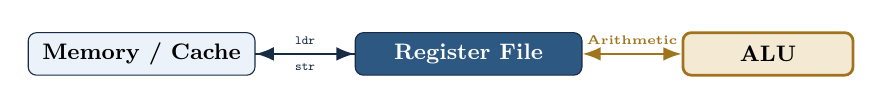
\begin{tikzpicture}[scale=0.9, every node/.style={transform shape}]
  \node[draw=navy, fill=lightblue, rounded corners=3pt, font=\small\bfseries, minimum width=3.2cm, minimum height=0.6cm] (mem) {Memory / Cache};
  \node[draw=navy, fill=deepblue, text=white, rounded corners=3pt, font=\small\bfseries, right=1.4cm of mem, minimum width=3.2cm, minimum height=0.6cm] (reg) {Register File};
  \node[draw=gold!80!black, fill=gold!20, line width=1pt, rounded corners=3pt, font=\small\bfseries, right=1.4cm of reg, minimum width=2.4cm, minimum height=0.6cm] (alu) {ALU};

  \draw[-{Latex}, thick, navy] (mem) -- (reg) node[midway, above, font=\tiny\bfseries] {\code{ldr}};
  \draw[-{Latex}, thick, navy] (reg) -- (mem) node[midway, below, font=\tiny\bfseries] {\code{str}};
  \draw[{Latex}-{Latex}, thick, gold!80!black] (reg) -- (alu) node[midway, above, font=\tiny\bfseries] {Arithmetic};
\end{tikzpicture}
\end{frame}

% ============================================================
% Slide 5
% ============================================================

\begin{frame}{Comparing Memory Models: RISC vs.\ CISC}
\begin{columns}[T,onlytextwidth]
\begin{column}{0.48\textwidth}
\begin{block}{AArch64 (Explicit Load/Store)}
\small
\begin{tabular}{ll}
\code{ldr x1, [x0]}   & \text{\scriptsize // Load from address in x0} \\
\code{add x2, x2, x1} & \text{\scriptsize // Compute in registers} \\
\code{str x2, [x0]}   & \text{\scriptsize // Write result back} \\
\end{tabular}
\vspace{0.15cm}
\begin{itemize}\setlength{\itemsep}{2pt}
  \item 3 simple, orthogonal instructions.
  \item Compiler can schedule other work during memory load latency.
\end{itemize}
\end{block}
\end{column}

\begin{column}{0.48\textwidth}
\begin{block}{x86-64 (Register-Memory CISC)}
\small
\begin{tabular}{ll}
\code{add [rdi], rax} & \text{\scriptsize // Memory Read-Modify-Write} \\
\end{tabular}
\vspace{0.15cm}
\begin{itemize}\setlength{\itemsep}{2pt}
  \item 1 complex instruction.
  \item Hardware decoder must split this internally into multiple micro-operations.
\end{itemize}
\end{block}
\end{column}
\end{columns}

\vspace{0.35cm}
\normalsize
\key{Takeaway:} RISC exposes data movement directly to the compiler rather than hiding it inside complex hardware decoders.
\end{frame}

% ============================================================
% Slide 6
% ============================================================

\begin{frame}{Addressing Memory: Bytes, Words, and Doublewords}
\large
\begin{itemize}\setlength{\itemsep}{6pt}
  \item Memory is a linear sequence of \key{8-bit bytes}, each with a unique 64-bit address.
  \item AArch64 uses register naming to determine the size of the memory transaction:
\end{itemize}

\vspace{0.2cm}
\begin{center}
\small
\setlength{\tabcolsep}{8pt}
\begin{tabular}{lccc}
\toprule
\textbf{Data Type} & \textbf{Width} & \textbf{Load Syntax} & \textbf{Store Syntax} \\
\midrule
Byte         & 8-bit   & \code{ldrb wt, [xn]} & \code{strb wt, [xn]} \\
Halfword     & 16-bit  & \code{ldrh wt, [xn]} & \code{strh wt, [xn]} \\
Word         & 32-bit  & \code{ldr  wt, [xn]} & \code{str  wt, [xn]} \\
Doubleword   & 64-bit  & \code{ldr  xt, [xn]} & \code{str  xt, [xn]} \\
\bottomrule
\end{tabular}
\end{center}

\vspace{0.25cm}
\normalsize
The base register (\bits{xn}) holds the 64-bit memory pointer enclosed in brackets: \code{[xn]}.
\end{frame}

% ============================================================
% Section 2 Divider
% ============================================================

\sectiondivider{PART 2}{Data Sizing \& Extension Rules}

% ============================================================
% Slide 7
% ============================================================

\begin{frame}{The Sub-Word Loading Problem}
\large
\begin{itemize}\setlength{\itemsep}{7pt}
  \item Registers are 64 bits wide, but data items in memory are often 8 bits or 16 bits.
  \item When an 8-bit byte is loaded into a 64-bit register, \key{what happens to the remaining 56 bits?}
  \item The answer depends on whether the data is \key{unsigned} (e.g., characters, raw bytes) or \key{signed} (e.g., small integers).
\end{itemize}

\vspace{0.3cm}
\begin{columns}[T,onlytextwidth]
\begin{column}{0.48\textwidth}
\begin{block}{Unsigned Data (Zero-Extension)}
Fill all upper bits with \bits{0}s to preserve magnitude.
\end{block}
\end{column}

\begin{column}{0.48\textwidth}
\begin{block}{Signed Data (Sign-Extension)}
Replicate the sign bit to preserve negative values.
\end{block}
\end{column}
\end{columns}
\end{frame}

% ============================================================
% Slide 8
% ============================================================

\begin{frame}{Unsigned Loads: Automatic Zero-Extension}
\large
\begin{itemize}\setlength{\itemsep}{6pt}
  \item Standard sub-word loads (\code{ldrb}, \code{ldrh}, \code{ldr wt}) \key{automatically clear all upper bits to zero}.
\end{itemize}

\vspace{0.2cm}
\centering
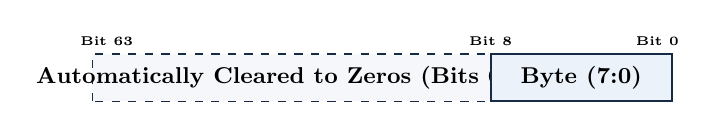
\begin{tikzpicture}[scale=0.92, every node/.style={transform shape}]
  \draw[fill=softgray, draw=navy, dashed] (0,0) rectangle (5.5,0.65);
  \node at (2.75, 0.325) {\small\textbf{Automatically Cleared to Zeros (Bits 63:8)}};
  \draw[fill=lightblue, draw=navy, thick] (5.5,0) rectangle (8.0,0.65);
  \node at (6.75, 0.325) {\small\textbf{Byte (7:0)}};
  \node[anchor=south, font=\tiny\bfseries] at (0.2, 0.65) {Bit 63};
  \node[anchor=south, font=\tiny\bfseries] at (5.5, 0.65) {Bit 8};
  \node[anchor=south, font=\tiny\bfseries] at (7.8, 0.65) {Bit 0};
\end{tikzpicture}

\vspace{0.3cm}
\begin{block}{Example: Loading Byte \hex{80}}
\small
\begin{tabular}{lll}
\code{ldrb w0, [x1]} & $\implies x_0 = \hex{00000000\_00000080} = +128_{10}$ & (Unsigned integer) \\
\end{tabular}
\end{block}
\end{frame}

% ============================================================
% Slide 9
% ============================================================

\begin{frame}{Signed Loads: Sign-Extension (\texttt{ldrsb}, \texttt{ldrsh}, \texttt{ldrsw})}
\large
\begin{itemize}\setlength{\itemsep}{6pt}
  \item The ``\code{s}'' in \code{ldrsb}, \code{ldrsh}, and \code{ldrsw} stands for \key{Signed Load}.
  \item Copies the sign bit across all upper bits up to the destination width.
\end{itemize}

\vspace{0.2cm}
\centering
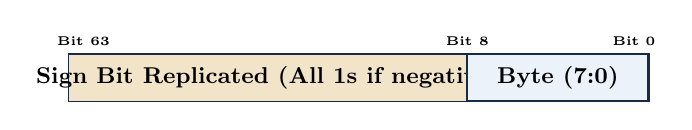
\begin{tikzpicture}[scale=0.92, every node/.style={transform shape}]
  \draw[fill=gold!25, draw=navy] (0,0) rectangle (5.5,0.65);
  \node at (2.75, 0.325) {\small\textbf{Sign Bit Replicated (All 1s if negative)}};
  \draw[fill=lightblue, draw=navy, thick] (5.5,0) rectangle (8.0,0.65);
  \node at (6.75, 0.325) {\small\textbf{Byte (7:0)}};
  \node[anchor=south, font=\tiny\bfseries] at (0.2, 0.65) {Bit 63};
  \node[anchor=south, font=\tiny\bfseries] at (5.5, 0.65) {Bit 8};
  \node[anchor=south, font=\tiny\bfseries] at (7.8, 0.65) {Bit 0};
\end{tikzpicture}

\vspace{0.3cm}
\begin{block}{Example: Loading Byte \hex{80} ($-128$ in 8-bit signed)}
\small
\begin{tabular}{lll}
\code{ldrsb x0, [x1]} & $\implies x_0 = \hex{ffffffff\_ffffff80} = -128_{10}$ & (Sign preserved in 64 bits) \\
\end{tabular}
\end{block}
\end{frame}

% ============================================================
% Slide 10
% ============================================================

\begin{frame}{Sign vs.\ Zero Extension: Side-by-Side}
\begin{block}{Memory Byte at Address \texttt{x1} = \hex{80} (Binary: \texttt{1000 0000})}
\end{block}

\vspace{0.15cm}
\begin{center}
\footnotesize
\setlength{\tabcolsep}{6pt}
\begin{tabular}{ll>{\raggedright\arraybackslash}p{5.5cm}}
\toprule
\textbf{Executed Instruction} & \textbf{64-bit Hex in \texttt{x0}} & \textbf{Decimal Value and Meaning} \\
\midrule
\code{ldrb  w0, [x1]} & \texttt{0x00000000\_00000080} & $+128$ (Unsigned zero-extension) \\[0.3em]
\code{ldrsb w0, [x1]} & \texttt{0x00000000\_ffffff80} & $-128$ (Sign-extended to 32b, upper zeroed) \\[0.3em]
\code{ldrsb x0, [x1]} & \texttt{0xffffffff\_ffffff80} & $-128$ (Sign-extended to full 64b) \\
\bottomrule
\end{tabular}
\end{center}

\vspace{0.25cm}
\normalsize
\begin{block}{Common Bug}
Using \code{ldrb} on a signed negative variable results in a large positive number, causing if-statements and comparisons to fail unexpectedly.
\end{block}
\end{frame}

% ============================================================
% Slide 11
% ============================================================

\begin{frame}{Storing Data: Truncation Rules}
\large
\begin{itemize}\setlength{\itemsep}{6pt}
  \item Stores move data from a register into memory.
  \item The instruction width determines how many bytes from the register are written:
\end{itemize}

\vspace{0.15cm}
\begin{center}
\small
\setlength{\tabcolsep}{8pt}
\begin{tabular}{lll}
\toprule
\textbf{Instruction} & \textbf{Bits Read from Register} & \textbf{Bytes Written to Memory} \\
\midrule
\code{strb wt, [xn]} & Bits [7:0]   & Writes exactly 1 byte \\
\code{strh wt, [xn]} & Bits [15:0]  & Writes exactly 2 bytes \\
\code{str  wt, [xn]} & Bits [31:0]  & Writes exactly 4 bytes \\
\code{str  xt, [xn]} & Bits [63:0]  & Writes full 8 bytes (doubleword) \\
\bottomrule
\end{tabular}
\end{center}

\vspace{0.25cm}
\normalsize
\key{Takeaway:} Storing a byte or halfword modifies \emph{only} the targeted memory locations without overwriting neighboring bytes.
\end{frame}

% ============================================================
% Section 3 Divider
% ============================================================

\sectiondivider{PART 3}{AArch64 Addressing Modes}

% ============================================================
% Slide 12
% ============================================================

\begin{frame}{What Is an Addressing Mode?}
\large
\begin{itemize}\setlength{\itemsep}{7pt}
  \item An \key{addressing mode} is the method used by an instruction to compute the \key{Effective Address (EA)} of a data operand in memory.
  \item Different data structures require different address calculations:
  \begin{itemize}\setlength{\itemsep}{4pt}
    \item Fixed struct members $\to$ \key{Base + Constant Offset}
    \item Sequential arrays $\to$ \key{Auto-Incrementing Pointers}
    \item Array indexing (\code{arr[i]}) $\to$ \key{Base + Scaled Register Index}
    \item Global variables $\to$ \key{PC-Relative Page Addressing}
  \end{itemize}
\end{itemize}
\end{frame}

% ============================================================
% Slide 13
% ============================================================

\begin{frame}{Mode 1: Base Register with Immediate Offset}

\begin{itemize}\setlength{\itemsep}{5pt}
  \item Adds a fixed constant to a base pointer without modifying the base register.
  \item \key{Syntax:} \code{ldr xt, [xn, \#offset]} $\implies \text{EA} = x_n + \text{offset}$.
\end{itemize}

\vspace{0.2cm}
\centering
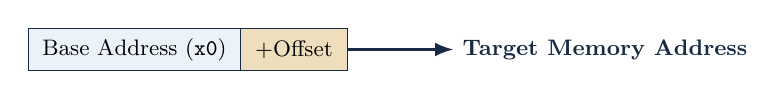
\begin{tikzpicture}[scale=0.9, every node/.style={transform shape}]
  \draw[fill=lightblue, draw=navy] (0,0) rectangle (3.0,0.6) node[midway, font=\small] {Base Address (\bits{x0})};
  \draw[fill=gold!30, draw=navy] (3.0,0) rectangle (4.5,0.6) node[midway, font=\small] {$+ \text{Offset}$};
  \draw[-{Latex}, thick, navy] (4.5,0.3) -- (6.0,0.3) node[right, font=\small\bfseries] {Target Memory Address};
\end{tikzpicture}

\vspace{0.3cm}
\begin{block}{Example: Reading Struct Fields}
\small
\begin{tabular}{ll}
\code{ldr x1, [x0, \#0]}  & \text{\scriptsize // Read field 1 at offset 0} \\
\code{ldr x2, [x0, \#8]}  & \text{\scriptsize // Read field 2 at offset 8} \\
\code{ldr w3, [x0, \#16]} & \text{\scriptsize // Read 32-bit field at offset 16} \\
\end{tabular}
\end{block}
\end{frame}

% ============================================================
% Slide 14
% ============================================================

\begin{frame}{Offset Scaling for Efficiency}
\large
\begin{itemize}\setlength{\itemsep}{6pt}
  \item In 32-bit instructions, immediate fields have limited bit width.
  \item AArch64 uses \key{scaled offsets} matching the operand size:
  \begin{itemize}\setlength{\itemsep}{3pt}
    \item 64-bit loads scale offsets by $\times 8$ ($0, 8, 16, \dots, 32760$).
    \item 32-bit loads scale offsets by $\times 4$ ($0, 4, 8, \dots, 16380$).
  \end{itemize}
  \item Allows instructions to reach up to $\approx 32\text{ KB}$ from a base pointer using only 12 encoding bits.
\end{itemize}

\vspace{0.25cm}
\begin{block}{Negative or Unaligned Offsets (\texttt{ldur}/\texttt{stur})}
If an offset is negative or unaligned, use unscaled load/store: \code{ldur xt, [xn, \#-8]}.
\end{block}
\end{frame}

% ============================================================
% Slide 15
% ============================================================

\begin{frame}{Mode 2: Pre-Indexed Addressing (Update Before Access)}

\begin{itemize}\setlength{\itemsep}{5pt}
  \item Updates the base register \key{before} reading or writing memory.
  \item \key{Syntax:} \code{ldr xt, [xn, \#offset]!} \quad (Exclamation mark indicates update).
\end{itemize}

\vspace{0.2cm}
\begin{block}{Step-by-Step Action}
\begin{enumerate}\setlength{\itemsep}{3pt}
  \item $x_n \leftarrow x_n + \text{offset}$ \quad (Update pointer)
  \item Access memory at the \key{new} address in $x_n$.
\end{enumerate}
\end{block}

\vspace{0.25cm}
\begin{block}{Primary Use Case: Stack Push}
\code{str x30, [sp, \#-16]!} \\
\text{\scriptsize Moves the stack pointer down by 16 bytes, then writes register x30 to the new top of stack.}
\end{block}
\end{frame}

% ============================================================
% Slide 16
% ============================================================

\begin{frame}{Mode 3: Post-Indexed Addressing (Update After Access)}

\begin{itemize}\setlength{\itemsep}{5pt}
  \item Reads or writes memory at the current address, then updates the base pointer \key{afterwards}.
  \item \key{Syntax:} \code{ldr xt, [xn], \#offset} \quad (Offset written outside the brackets).
\end{itemize}

\vspace{0.2cm}
\begin{block}{Step-by-Step Action}
\begin{enumerate}\setlength{\itemsep}{3pt}
  \item Access memory at the \key{current} address in $x_n$.
  \item $x_n \leftarrow x_n + \text{offset}$ \quad (Advance pointer)
\end{enumerate}
\end{block}

\vspace{0.25cm}
\begin{block}{Primary Use Case: Array Stepping \& Stack Pop}
\code{ldr x0, [x1], \#8} \\
\text{\scriptsize Loads data from current address in x1, then automatically advances x1 to the next 8-byte element.}
\end{block}
\end{frame}

% ============================================================
% Slide 17
% ============================================================

\begin{frame}{Comparing the Three Offset Modes}
\begin{center}
\small
\setlength{\tabcolsep}{6pt}
\begin{tabular}{llll}
\toprule
\textbf{Mode} & \textbf{Syntax Pattern} & \textbf{Address Accessed} & \textbf{Base Register After} \\
\midrule
\textbf{Standard Offset} & \code{[xn, \#8]}  & $x_n + 8$ & $x_n$ (Unchanged) \\
\textbf{Pre-Indexed}     & \code{[xn, \#8]!} & $x_n + 8$ & $x_n + 8$ (Updated) \\
\textbf{Post-Indexed}    & \code{[xn], \#8}  & $x_n$     & $x_n + 8$ (Updated) \\
\bottomrule
\end{tabular}
\end{center}

\vspace{0.3cm}
\begin{block}{Assume \texttt{x1} = \hex{1000} Initially}
\small
\begin{tabular}{llll}
\code{ldr x0, [x1, \#8]}  & $\implies$ Reads from \hex{1008}; & $x_1$ remains \hex{1000} \\
\code{ldr x0, [x1, \#8]!} & $\implies$ Reads from \hex{1008}; & $x_1$ becomes \hex{1008} \\
\code{ldr x0, [x1], \#8}  & $\implies$ Reads from \hex{1000}; & $x_1$ becomes \hex{1008} \\
\end{tabular}
\end{block}
\end{frame}

% ============================================================
% Slide 18
% ============================================================

\begin{frame}{Mode 4: Register Offset with Scaling}
\large
\begin{itemize}\setlength{\itemsep}{6pt}
  \item Uses an index register ($x_m$) multiplied by element size to access array items:
  $$\code{ldr xt, [xn, xm, lsl \#shift]}$$
  \item Hardware computes $\text{Base} + (\text{Index} \times \text{Size})$ with \key{zero extra cycle penalty}.
\end{itemize}

\vspace{0.2cm}
\begin{center}
\small
\setlength{\tabcolsep}{8pt}
\begin{tabular}{lll}
\toprule
\textbf{Array Element Type} & \textbf{Assembly Instruction} & \textbf{Effective Address} \\
\midrule
Byte (\code{uint8})    & \code{ldrb w0, [x1, x2]}          & $\text{EA} = x_1 + x_2$ \\
Halfword (\code{uint16})& \code{ldrh w0, [x1, x2, lsl \#1]} & $\text{EA} = x_1 + (x_2 \times 2)$ \\
Word (\code{uint32})    & \code{ldr  w0, [x1, x2, lsl \#2]} & $\text{EA} = x_1 + (x_2 \times 4)$ \\
Doubleword (\code{uint64})& \code{ldr  x0, [x1, x2, lsl \#3]} & $\text{EA} = x_1 + (x_2 \times 8)$ \\
\bottomrule
\end{tabular}
\end{center}

\vspace{0.2cm}
\normalsize
Directly implements high-level array access: \code{val = arr[i];}.
\end{frame}

% ============================================================
% Slide 19
% ============================================================

\begin{frame}{Mixing 32-bit Indices with 64-bit Pointers}
\large
\begin{itemize}\setlength{\itemsep}{6pt}
  \item In C code, loop counter variables are frequently 32-bit integers (\code{int i}).
  \item Memory addresses are always 64 bits.
  \item AArch64 can extend and scale a 32-bit index register in one step:
\end{itemize}

\vspace{0.2cm}
\begin{block}{Signed vs.\ Unsigned Indexing}
\small
\begin{tabular}{ll}
\code{ldr x0, [x1, w2, sxtw \#3]} & \text{\scriptsize // Sign-extend 32-bit index w2, multiply by 8, add to x1} \\
\code{ldr x0, [x1, w2, uxtw \#3]} & \text{\scriptsize // Zero-extend 32-bit index w2, multiply by 8, add to x1} \\
\end{tabular}
\end{block}

\vspace{0.25cm}
\normalsize
\key{Benefit:} Eliminates separate instructions to convert \code{int} indices to 64-bit pointers.
\end{frame}

% ============================================================
% Slide 20
% ============================================================

\begin{frame}{Mode 5: PC-Relative Global Variable Access}
\large
\begin{itemize}\setlength{\itemsep}{6pt}
  \item Modern programs use Position-Independent Code (PIC) so code can load anywhere in memory.
  \item Global variables are addressed relative to the current \key{Program Counter (\bits{pc})}.
  \item Access is performed in a clean two-step sequence:
\end{itemize}

\vspace{0.2cm}
\begin{block}{Loading a Global Variable}
\small
\begin{tabular}{ll}
\texttt{adrp x0, my\_global}             & \text{\scriptsize // Step 1: Form base address of the 4KB page} \\
\texttt{ldr  x1, [x0, :lo12:my\_global]} & \text{\scriptsize // Step 2: Add page offset and load value} \\
\end{tabular}
\end{block}

\vspace{0.25cm}
\normalsize
Can reach any global data variable within $\pm 4\text{ GB}$ of the current instruction.
\end{frame}

% ============================================================
% Slide 21
% ============================================================

\begin{frame}{PC-Relative Literal Pools}
\large
\begin{itemize}\setlength{\itemsep}{6pt}
  \item How do we load arbitrary 64-bit constants that cannot fit in an instruction?
  \item The compiler places the 64-bit constant in a \key{literal pool} near the code and uses a PC-relative load.
\end{itemize}

\vspace{0.2cm}
\begin{block}{Assembly Syntax}
\small
\begin{tabular}{ll}
\code{ldr x0, =0x0123456789abcdef} & \text{\scriptsize // Pseudo-instruction: compiler generates literal load} \\
\end{tabular}
\end{block}

\vspace{0.25cm}
\normalsize
The processor fetches the constant directly from the nearby text segment without runtime math.
\end{frame}

% ============================================================
% Section 4 Divider
% ============================================================

\sectiondivider{PART 4}{Multi-Register Transfers, Alignment, \& Stack}

% ============================================================
% Slide 22
% ============================================================

\begin{frame}{Paired Transfers: \texttt{ldp} and \texttt{stp}}
\large
\begin{itemize}\setlength{\itemsep}{6pt}
  \item AArch64 provides dedicated instructions to move \key{two registers in one command}:
  $$\code{ldp\quad x0,\; x1,\; [x2]} \qquad \code{stp\quad x0,\; x1,\; [x2]}$$
  \item Transfers 16 contiguous bytes across a 128-bit memory bus transaction.
\end{itemize}

\vspace{0.2cm}
\begin{center}
\small
\setlength{\tabcolsep}{8pt}
\begin{tabular}{lll}
\toprule
\textbf{Instruction} & \textbf{Action} & \textbf{Primary Use Case} \\
\midrule
\code{stp x29, x30, [sp, \#-16]!} & Push Frame Pointer \& Link Register & Function entry (prologue) \\
\code{ldp x29, x30, [sp], \#16}   & Restore FP \& LR, adjust stack      & Function exit (epilogue) \\
\code{ldp x0, x1, [x2]}           & Load two 64-bit values into x0, x1  & Fast struct/buffer copy \\
\bottomrule
\end{tabular}
\end{center}
\end{frame}

% ============================================================
% Slide 23
% ============================================================

\begin{frame}{Why Paired Transfers Matter}
\begin{columns}[T,onlytextwidth]
\begin{column}{0.48\textwidth}
\begin{block}{Individual Transfers}
\small
\begin{tabular}{l}
\code{str x29, [sp, \#-8]!} \\
\code{str x30, [sp, \#-8]!} \\
\end{tabular}
\vspace{0.15cm}
\begin{itemize}\setlength{\itemsep}{2pt}
  \item 2 instructions.
  \item 2 separate 64-bit bus requests.
  \item Breaks 16-byte stack alignment.
\end{itemize}
\end{block}
\end{column}

\begin{column}{0.48\textwidth}
\begin{block}{Paired Transfer}
\small
\begin{tabular}{l}
\code{stp x29, x30, [sp, \#-16]!} \\
\end{tabular}
\vspace{0.15cm}
\begin{itemize}\setlength{\itemsep}{2pt}
  \item 1 single instruction.
  \item 1 unified 128-bit bus transaction.
  \item Naturally maintains 16-byte stack alignment.
\end{itemize}
\end{block}
\end{column}
\end{columns}

\vspace{0.35cm}
\normalsize
\key{Efficiency Impact:} Cuts memory instructions in function prologues and epilogues by $50\%$.
\end{frame}

% ============================================================
% Slide 24
% ============================================================

\begin{frame}{Memory Alignment Principles}
\large
\begin{itemize}\setlength{\itemsep}{6pt}
  \item An access is \key{naturally aligned} if its memory address is an exact multiple of the data size:
  $$\text{Address} \pmod{\text{Data Size}} = 0$$
\end{itemize}

\vspace{0.2cm}
\begin{columns}[T,onlytextwidth]
\begin{column}{0.48\textwidth}
\begin{block}{Aligned Access}
\centering
\vspace{0.1cm}
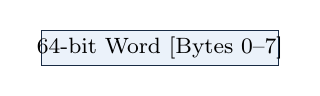
\begin{tikzpicture}[scale=0.75]
  \draw[fill=lightblue, draw=navy] (0,0) rectangle (4,0.6) node[midway, font=\footnotesize] {64-bit Word [Bytes 0--7]};
\end{tikzpicture}
\vspace{0.1cm}
Single memory transaction within one cache line. Fast and efficient.
\end{block}
\end{column}

\begin{column}{0.48\textwidth}
\begin{block}{Unaligned Access}
\centering
\vspace{0.1cm}
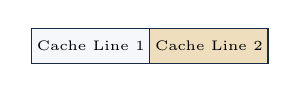
\begin{tikzpicture}[scale=0.75]
  \draw[fill=softgray, draw=navy] (0,0) rectangle (2,0.6) node[midway, font=\tiny] {Cache Line 1};
  \draw[fill=gold!30, draw=navy] (2,0) rectangle (4,0.6) node[midway, font=\tiny] {Cache Line 2};
\end{tikzpicture}
\vspace{0.1cm}
Crosses boundary. Requires two memory cycles and extra logic to stitch data.
\end{block}
\end{column}
\end{columns}
\end{frame}

% ============================================================
% Slide 25
% ============================================================

\begin{frame}{Stack Alignment: A Strict Architectural Rule}
\large
\begin{itemize}\setlength{\itemsep}{7pt}
  \item The AArch64 ABI strictly enforces \key{16-byte alignment on the Stack Pointer (\bits{sp})}.
  \item Any memory operation using \bits{sp} when $\bits{sp} \pmod{16} \neq 0$ triggers a hardware alignment exception.
  \item When allocating local variables or saving registers, total stack space must always be padded to a multiple of 16 bytes.
\end{itemize}

\vspace{0.3cm}
\begin{block}{Correct Stack Adjustment Example}
\small
\begin{tabular}{lll}
\code{sub sp, sp, \#16} & \text{\scriptsize // Correct: 16-byte multiple} \\
\code{sub sp, sp, \#32} & \text{\scriptsize // Correct: 32-byte multiple} \\
\code{sub sp, sp, \#8}  & \text{\scriptsize // ERROR: Violates 16-byte alignment!} \\
\end{tabular}
\end{block}
\end{frame}

% ============================================================
% Slide 26
% ============================================================

\begin{frame}[fragile]{Standard Function Stack Frame Layout}
\begin{columns}[T,onlytextwidth]
\begin{column}{0.50\textwidth}
\begin{block}{Function Code}
\small
\begin{verbatim}
my_func:
    // 1. Save Frame Pointer & Link Reg
    // Allocate 32 bytes total
    stp  x29, x30, [sp, #-32]!
    mov  x29, sp

    // 2. Save callee-saved register
    str  x19, [sp, #16]

    // ... Function body ...

    // 3. Restore and return
    ldr  x19, [sp, #16]
    ldp  x29, x30, [sp], #32
    ret
\end{verbatim}
\end{block}
\end{column}

\begin{column}{0.44\textwidth}
\centering
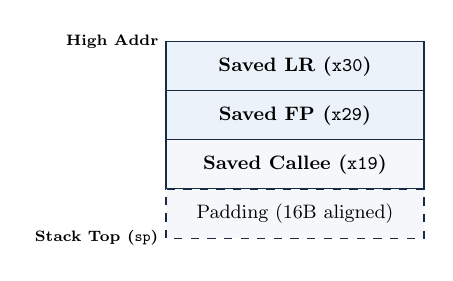
\begin{tikzpicture}[scale=0.78, every node/.style={transform shape}]
  \draw[fill=lightblue, draw=navy] (0,3.6) rectangle (4.2,4.4) node[midway, font=\small\bfseries] {Saved LR (\bits{x30})};
  \draw[fill=lightblue, draw=navy] (0,2.8) rectangle (4.2,3.6) node[midway, font=\small\bfseries] {Saved FP (\bits{x29})};
  \draw[fill=softgray, draw=navy] (0,2.0) rectangle (4.2,2.8) node[midway, font=\small\bfseries] {Saved Callee (\bits{x19})};
  \draw[fill=softgray, draw=navy, dashed] (0,1.2) rectangle (4.2,2.0) node[midway, font=\small] {Padding (16B aligned)};
  \node[anchor=east, font=\scriptsize\bfseries] at (0,4.4) {High Addr};
  \node[anchor=east, font=\scriptsize\bfseries] at (0,1.2) {Stack Top (\bits{sp})};
\end{tikzpicture}
\end{column}
\end{columns}
\end{frame}

% ============================================================
% Slide 27
% ============================================================

\begin{frame}[fragile]{Worked Pattern 1: Stepping Through an Array}
\begin{block}{Goal: Sum $N$ 64-bit Integers}
\end{block}

\vspace{0.1cm}
\begin{block}{AArch64 Implementation (Using Post-Indexed Addressing)}
\small
\begin{tabular}{lll}
\multicolumn{3}{l}{\textit{// x0 = array pointer, x1 = count n}} \\
\code{sum\_loop:} & & \\
    & \code{mov  x2, xzr}           & \text{\scriptsize // sum = 0} \\
    & \code{cbz  x1, .Ldone}        & \text{\scriptsize // Exit if count == 0} \\
\code{.Lbody:} & & \\
    & \code{ldr  x3, [x0], \#8}     & \text{\scriptsize // Load element AND increment pointer by 8} \\
    & \code{add  x2, x2, x3}        & \text{\scriptsize // sum += element} \\
    & \code{subs x1, x1, \#1}       & \text{\scriptsize // count--} \\
    & \code{cbnz x1, .Lbody}        & \text{\scriptsize // Loop if count != 0} \\
\code{.Ldone:} & & \\
    & \code{mov  x0, x2}           & \text{\scriptsize // Return sum in x0} \\
    & \code{ret}                    & \\
\end{tabular}
\end{block}

\vspace{0.15cm}
\normalsize
Post-indexing eliminates a separate \code{add x0, x0, \#8} instruction inside the loop.
\end{frame}

% ============================================================
% Slide 28
% ============================================================

\begin{frame}[fragile]{Worked Pattern 2: Indexed Array Search}
\begin{block}{Goal: Check Element at Index $i$ in Array}
\end{block}

\vspace{0.1cm}
\begin{block}{AArch64 Implementation (Using Scaled Register Offset)}
\small
\begin{tabular}{lll}
\multicolumn{3}{l}{\textit{// x0 = array pointer, x1 = index i, x2 = target value}} \\
\code{find\_element:} & & \\
    & \code{ldr  x3, [x0, x1, lsl \#3]} & \text{\scriptsize // Load arr[i] using Base + (i * 8)} \\
    & \code{cmp  x3, x2}                & \text{\scriptsize // Compare arr[i] with target} \\
    & \code{cset w0, eq}                & \text{\scriptsize // w0 = 1 if match, else 0} \\
    & \code{ret}                        & \\
\end{tabular}
\end{block}

\vspace{0.25cm}
\normalsize
Combines index scaling and load into a single instruction without modifying the base pointer \bits{x0}.
\end{frame}

% ============================================================
% Slide 29
% ============================================================

\begin{frame}[fragile]{Worked Pattern 3: Copying a Data Block}
\begin{block}{Goal: Copy 32 Bytes from Source to Destination}
\end{block}

\vspace{0.1cm}
\begin{block}{AArch64 Implementation (Using Paired Transfers)}
\small
\begin{tabular}{lll}
\multicolumn{3}{l}{\textit{// x0 = destination pointer, x1 = source pointer}} \\
\code{copy\_32\_bytes:} & & \\
    & \code{ldp  x2, x3, [x1]}       & \text{\scriptsize // Load first 16 bytes (two doublewords)} \\
    & \code{ldp  x4, x5, [x1, \#16]} & \text{\scriptsize // Load next 16 bytes} \\
    & \code{stp  x2, x3, [x0]}       & \text{\scriptsize // Store first 16 bytes} \\
    & \code{stp  x4, x5, [x0, \#16]} & \text{\scriptsize // Store next 16 bytes} \\
    & \code{ret}                     & \\
\end{tabular}
\end{block}

\vspace{0.25cm}
\normalsize
Moves 32 bytes of memory in just 4 instructions using dual-register operations.
\end{frame}

% ============================================================
% Slide 30
% ============================================================

\begin{frame}{Addressing Mode Selection Guide}
\begin{center}
\small
\setlength{\tabcolsep}{6pt}
\begin{tabular}{lll}
\toprule
\textbf{Programming Scenario} & \textbf{Best Addressing Mode} & \textbf{Example Instruction} \\
\midrule
Accessing Struct Field        & Base + Immediate Offset       & \code{ldr x1, [x0, \#8]} \\
Pushing to Stack              & Pre-Indexed Auto-Update       & \code{str x30, [sp, \#-16]!} \\
Popping from Stack            & Post-Indexed Auto-Update      & \code{ldr x30, [sp], \#16} \\
Sequential Array Stepping     & Post-Indexed Auto-Update      & \code{ldr x2, [x0], \#8} \\
Random Array Index (\code{a[i]})& Scaled Register Offset     & \code{ldr x2, [x0, x1, lsl \#3]} \\
Global Variable Reference     & PC-Relative Page Offset       & \code{adrp} $+$ \code{ldr} \\
\bottomrule
\end{tabular}
\end{center}
\end{frame}

% ============================================================
% Slide 31
% ============================================================

\begin{frame}{Hardware Memory Access: The Cache Line View}
\large
\begin{itemize}\setlength{\itemsep}{6pt}
  \item Hardware does not fetch individual bytes from DRAM; it fetches \key{64-byte Cache Lines}.
  \item \key{Spatial Locality:} Accessing contiguous memory (e.g., sequential array stepping) ensures data for subsequent loads is already in L1 cache.
  \item Choosing sequential addressing modes helps the processor hardware prefetcher predict memory access patterns accurately.
\end{itemize}

\vspace{0.25cm}
\begin{block}{Performance Insight}
Sequential post-indexed access patterns maximize cache line utilization, running significantly faster than scattered random access.
\end{block}
\end{frame}

% ============================================================
% Slide 32
% ============================================================

\begin{frame}{Common Memory Access Mistakes}
\large
\begin{itemize}\setlength{\itemsep}{6pt}
  \item \key{Wrong Sizing:} Using \code{ldr} (64-bit) instead of \code{ldr wt} (32-bit) on an array of integers reads adjacent memory as garbage.
  \item \key{Missing Sign Extension:} Using \code{ldrb} instead of \code{ldrsb} on negative numbers corrupts signed comparisons.
  \item \key{Incorrect Shift Scale:} Using \code{lsl \#2} instead of \code{lsl \#3} on an array of 64-bit pointers accesses the wrong memory location.
  \item \key{Stack Misalignment:} Adjusting \bits{sp} by non-16-byte multiples triggers hardware crashes.
\end{itemize}
\end{frame}

% ============================================================
% Section 5 Divider
% ============================================================

\sectiondivider{SUMMARY \& ASSESSMENT}{Review and Self-Test Questions}

% ============================================================
% Slide 33: Comprehensive Summary
% ============================================================

\begin{frame}{Topic 5: Comprehensive Summary}

\begin{itemize}\setlength{\itemsep}{5pt}
  \item \key{RISC Load/Store Discipline:} Arithmetic operations are strictly decoupled from memory; only explicit \code{ldr}/\code{str} touch memory.
  \item \key{Data Widths \& Extensions:} Sub-word loads zero-extend by default; signed data requires explicit \code{ldrsb}, \code{ldrsh}, or \code{ldrsw} to preserve negative values.
  \item \key{Core Addressing Modes:}
  \begin{itemize}\setlength{\itemsep}{1.5pt}
    \item Standard offset (\code{[xn, \#imm]}): Base remains unchanged.
    \item Pre-indexed (\code{[xn, \#imm]!}): Base updated before access (push).
    \item Post-indexed (\code{[xn], \#imm}): Base updated after access (pop / loop step).
    \item Scaled register offset (\code{[xn, xm, lsl \#3]}): Hardware array indexing.
  \end{itemize}
  \item \key{Paired Transfers \& Stack Alignment:} \code{ldp}/\code{stp} move 16 bytes per instruction; stack pointer must maintain 16-byte alignment.
\end{itemize}

\end{frame}

% ============================================================
% Slide 34: Self-Test Questions (Part 1)
% ============================================================

\begin{frame}{Self-Test Questions: Sizing \& Addressing Modes}

\begin{enumerate}\setlength{\itemsep}{7pt}
  \item \key{Sign Extension vs.\ Zero Extension:} Memory byte at address \hex{2000} holds value \hex{fe} ($-2$ in signed 8-bit). What value resides in register \bits{x0} after:
  \begin{itemize}\setlength{\itemsep}{2pt}
    \item \code{ldrb  w0, [x1]} \quad (where $x_1 = \hex{2000}$)
    \item \code{ldrsb x0, [x1]} \quad (where $x_1 = \hex{2000}$)
  \end{itemize}

  \item \key{Addressing Mode Mechanics:} If register \bits{x1} holds address \hex{3000}, what address is read and what is the final value in \bits{x1} for:
  \begin{itemize}\setlength{\itemsep}{2pt}
    \item \code{ldr x0, [x1, \#8]}
    \item \code{ldr x0, [x1, \#8]!}
    \item \code{ldr x0, [x1], \#8}
  \end{itemize}

  \item \key{Array Element Indexing:} Given base array pointer in \bits{x0} and index $i$ in \bits{x1}, write a single instruction to load a 32-bit integer \texttt{arr[i]} into \bits{w2}.
\end{enumerate}

\end{frame}

% ============================================================
% Slide 35: Self-Test Questions (Part 2)
% ============================================================

\begin{frame}{Self-Test Questions: Stack Alignment \& Paired Transfers}

\begin{enumerate}\setlength{\itemsep}{7pt}
  \item \key{Paired Stack Operation:} Explain what happens during the instruction:
  $$\code{stp x29, x30, [sp, \#-16]!}$$
  How does \bits{sp} change, and where are \bits{x29} and \bits{x30} stored?

  \item \key{Stack Alignment Enforcement:} Why does AArch64 require the stack pointer to be 16-byte aligned even when storing a single 8-byte register?

  \item \key{Position-Independent Code:} Why does loading a global variable address in AArch64 require a page-relative instruction (\code{adrp}) followed by an offset load?
\end{enumerate}

\end{frame}

\end{document}